\ylDisplay{Aku laadimine} % Ülesande nimi
{Valter Kiisk} % Autor
{piirkonnavoor} % Voor
{2008} % Aasta
{G 8} % Ülesande nr.
{7} % Raskustase
{
% Teema: Elektriahelad
\ifStatement
Teatava akumulaatori elektromotoorjõud kasvab laadimise käigus nõnda, nagu kujutatud joonisel. Samas on toodud ka elektriskeem, mida Juku kavatseb kasutada sellise akumulaatori laadimiseks. Pingeallika klemmidel on pinge \SI{6}{V}. Nii pingeallika kui ka aku sisetakistuse võib lugeda tühiseks. Kuidas peaks Juku valima takistite $R_1$ ja $R_2$ väärtused, kui ta taotleb, et maksimaalne laadimisvool ei ületaks \SI{100}{mA} ja laadimisvool muutuks nulliks, kui akumulaator on täielikult laetud? 

\begin{center}
	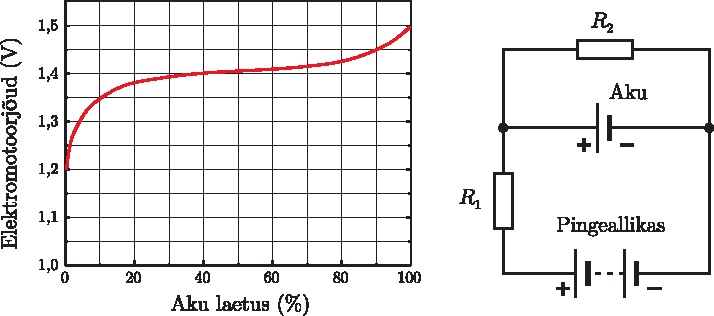
\includegraphics[width=\linewidth]{2008-v2g-08-yl}
\end{center}
\fi


\ifHint
Mõlema ülesandes antud tingimuse jaoks on võimalik kirja panna vastav võrrand (kasutades näiteks Kirchhoffi seadusi) ning saadud võrrandisüsteemi lahendid peaksidki olema $R_1$ ja $R_2$.
\fi


\ifSolution
Olgu aku klemmide pinge $U$ ning voolutugevuse $I$. Voolutugevus takistis $R_2$ on seega $U/R_2$ ja voolutugevus takistis $R_1$ avaldub kui $U/R_2 + I$. Teise Kirchhoffi seaduse kohaselt 
\[
U+\left(\frac{U}{R_{2}}+I\right) R_{1}=U_{0} \quad \Rightarrow \quad U R_{1}-\left(U_{0}-U\right) R_{2}+I R_{1} R_{2}=0,
\]
kus $U_0 = \SI{6}{V}$. Laadimisgraafikult leiame, et maksimaalne vool $I = \SI{0,1}{A}$ vastab pingele $U = \SI{1,2}{V}$, kui aga $U = \SI{1,5}{V}$ siis peab olema $I = 0$. Seega $R_1$ ja $R_2$ määramiseks saame võrrandisüsteemi 
\[
\num{1,2}R_1 - \num{4,8}R_2 + \num{0,1}R_1R_2 = 0, \quad \num{1,5}R_1 - \num{4,5}R_2 = 0. 
\]
Selle lahend on $R_1 = \SI{12}{\ohm}, R_2 = \SI{4}{\ohm}$.
\fi
}